%----------------------------------------------------------------------------------------
%	SLIDE 3.
%----------------------------------------------------------------------------------------
\begin{frame}
\frametitle{Simulations in Geant4}
\framesubtitle{Very short outline}

\begin{block}{Usual components}
	\begin{itemize}
		\item Detector construction
		\item Particle generation
		\item Data I/O
		\item Core loop
	\end{itemize}
\end{block}

%\begin{figure}
%	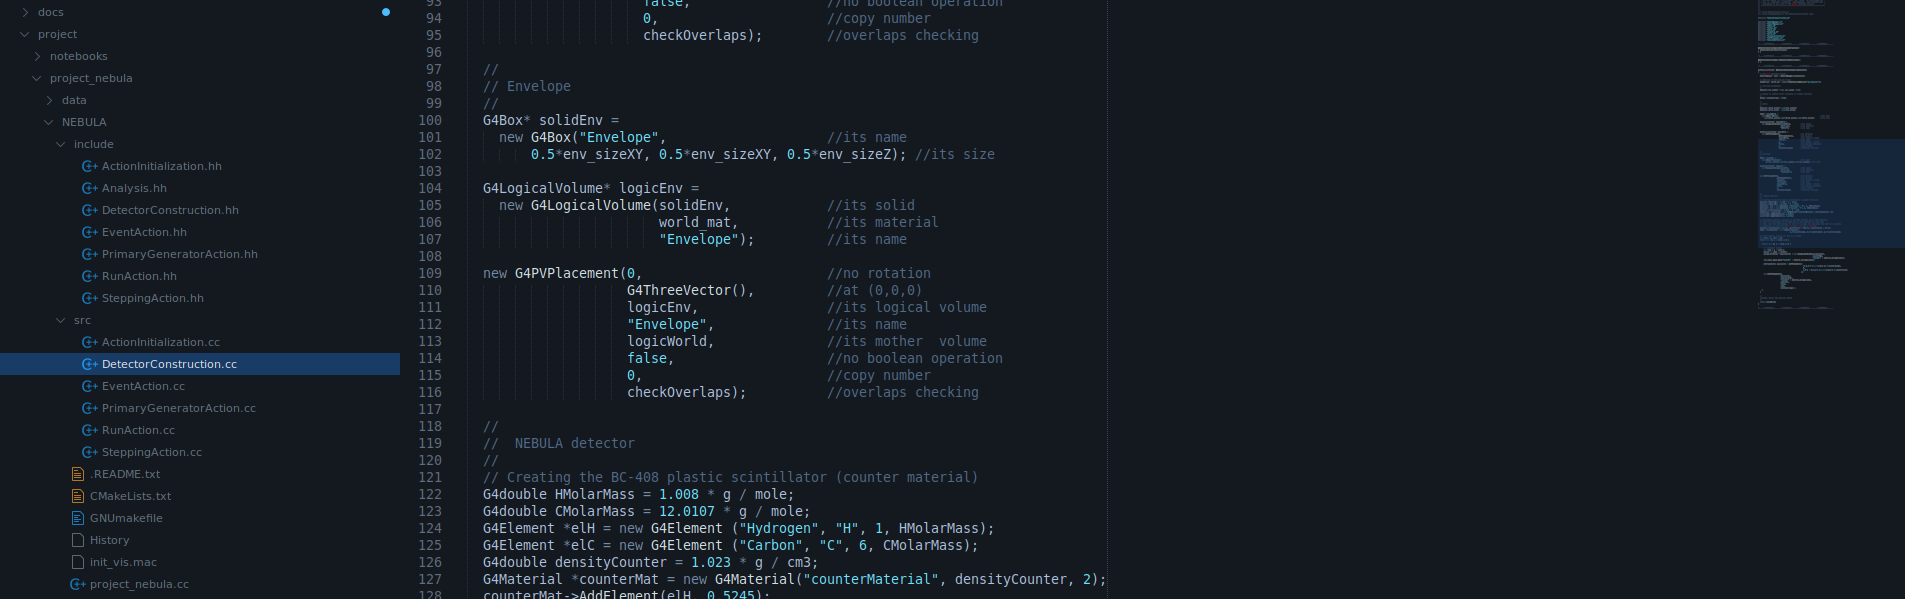
\includegraphics[width=0.9\textwidth]{images/nebula_code.png}
%\end{figure}

\begin{center}
	\begin{tikzpicture}
		\sbox0{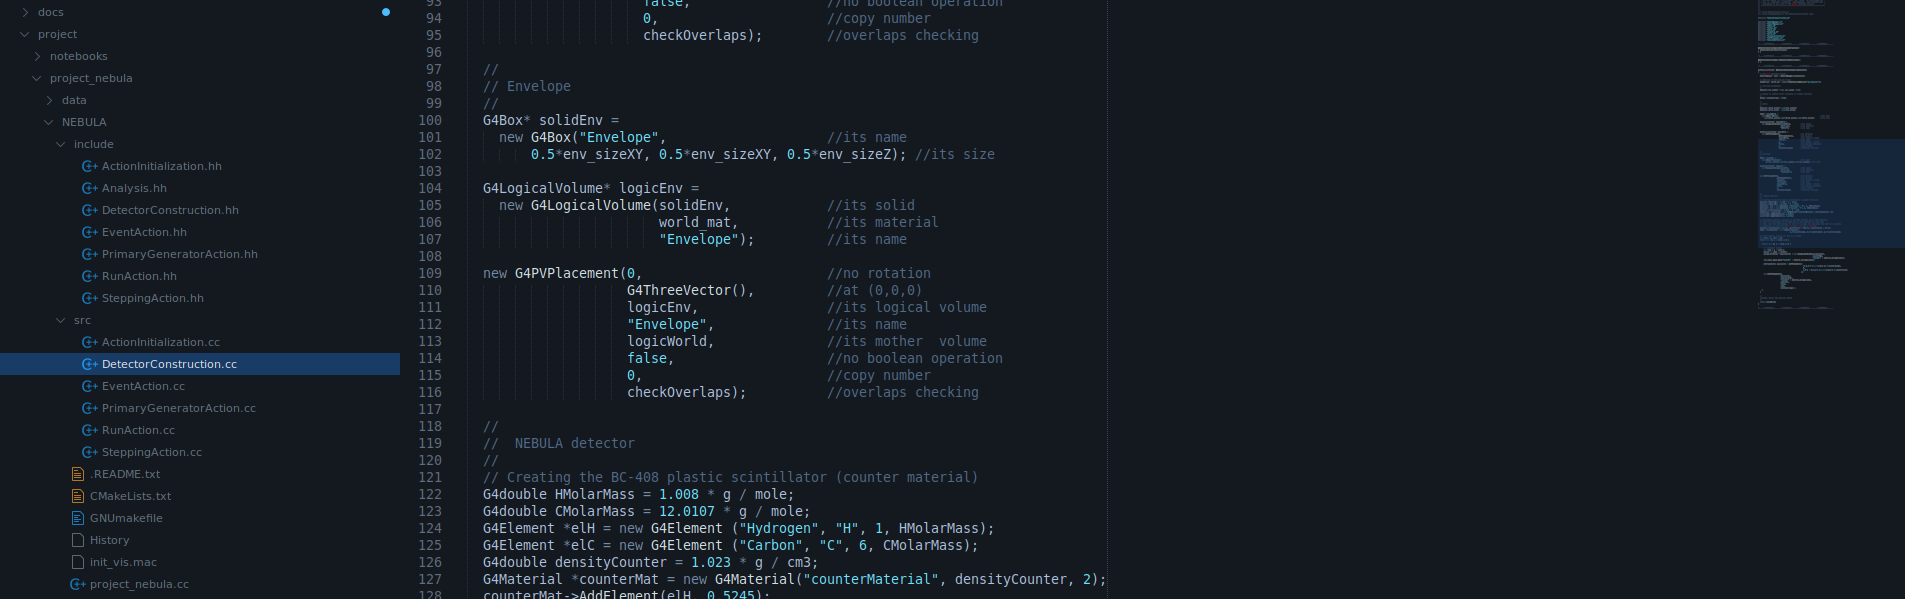
\includegraphics[width=0.95\textwidth]{images/nebula_code.png}}
		\path[clip,draw,rounded corners=0.3cm] (0,0) rectangle (\wd0,\ht0);
		\path (0.5\wd0,0.5\ht0) node[inner sep=0pt]{\usebox0};
	\end{tikzpicture}
\end{center}

\end{frame}